\section{\textsf{Fork}: Contribute to an existing repo}


\begin{figure} %[htp]
    \centering
    \begin{tikzpicture}
    \sbox0{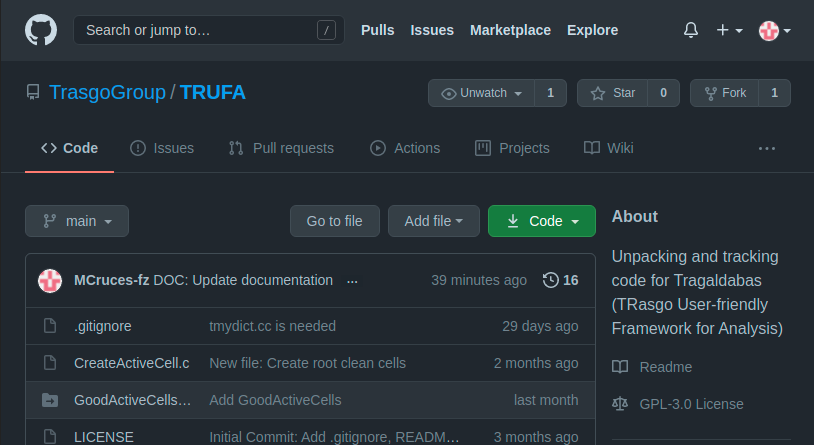
\includegraphics[width=\linewidth]{how_to_fork.png}}%
    \path[clip,rounded corners=10pt] (0,0) rectangle (\wd0,\ht0);
    \path (0.5\wd0,0.5\ht0) node[inner sep=0pt]{\usebox0};
    \end{tikzpicture}
    \caption{Example of main page of a repository.}
    \label{fig:Fork}
\end{figure}

Navigate to the repository which you want to fork using your web browser, and fork it to you account by clicking in the \textsf{Fork} button, shown in Figure \ref{fig:Fork}. The button is in the top-right corner of the page. If you belong to any organization, \textsf{GitHub} will ask you \textit{Where should we fork ``reponame''?} and you must choose the profile where you want to have said repository.

Once you have forked it, you can navigate to your \textsf{GitHub} profile and go to your repositories. If you open the forked repository you will see something similar to Figure \ref{fig:Fork}, then you are able to clone your forked repository by clicking in the green button \textsf{Code} and copying the \textsc{https} link.

You can clone this reposiroty from your \textsf{GitHub} account:
\begin{lstlisting}[style=shell]
cd <work_dir>
git clone <copied_link>
\end{lstlisting}
directly. Now you can edit, \texttt{git add}, \texttt{git commit}, \texttt{git push} and all you want.

